\documentclass[../main.tex]{subfiles}
\begin{document}
\chapter{Evaluation}
As described in Chapter \ref{chapter:impl}, the editor has been carefully designed to implement both the required and optional features. Two methods were used to determine how well the features are implemented: user feedback and automated testing.

\section{User Feedback}
\subsection{Collecting user feedback}
User feedback was collected through a survey form. The survey form, like the editor, was designed with people new to Logical English in mind. The form guided the responder through writing a preset Logical English program, constructed so that the responder would encounter the editor's features sequentially. Once the responder met each feature, they were asked to rate the feature by its intuitiveness and usefulness. At the end of the form, the responder was invited to suggest issues or points of improvement for the editor.

\subsection{Feedback Scores}
The survey form was filled out by seven people, none of whom had used Logical English before. The responders varied in programming ability: three had no experience in programming, one had limited experience, and the other three were confident student or professional programmers. Both groups benefited the survey. Those who were experienced in programming could judge the editor's features against editors they had used for other programming languages, while those with limited programming experience would judge the intuitiveness of the editor from a fresh perspective, with little prior experience to guide them to how to use certain features.
\\
\\
Figure \ref{fig:scores} shows the scores obtained.
\begin{figure}[h!]
\centering
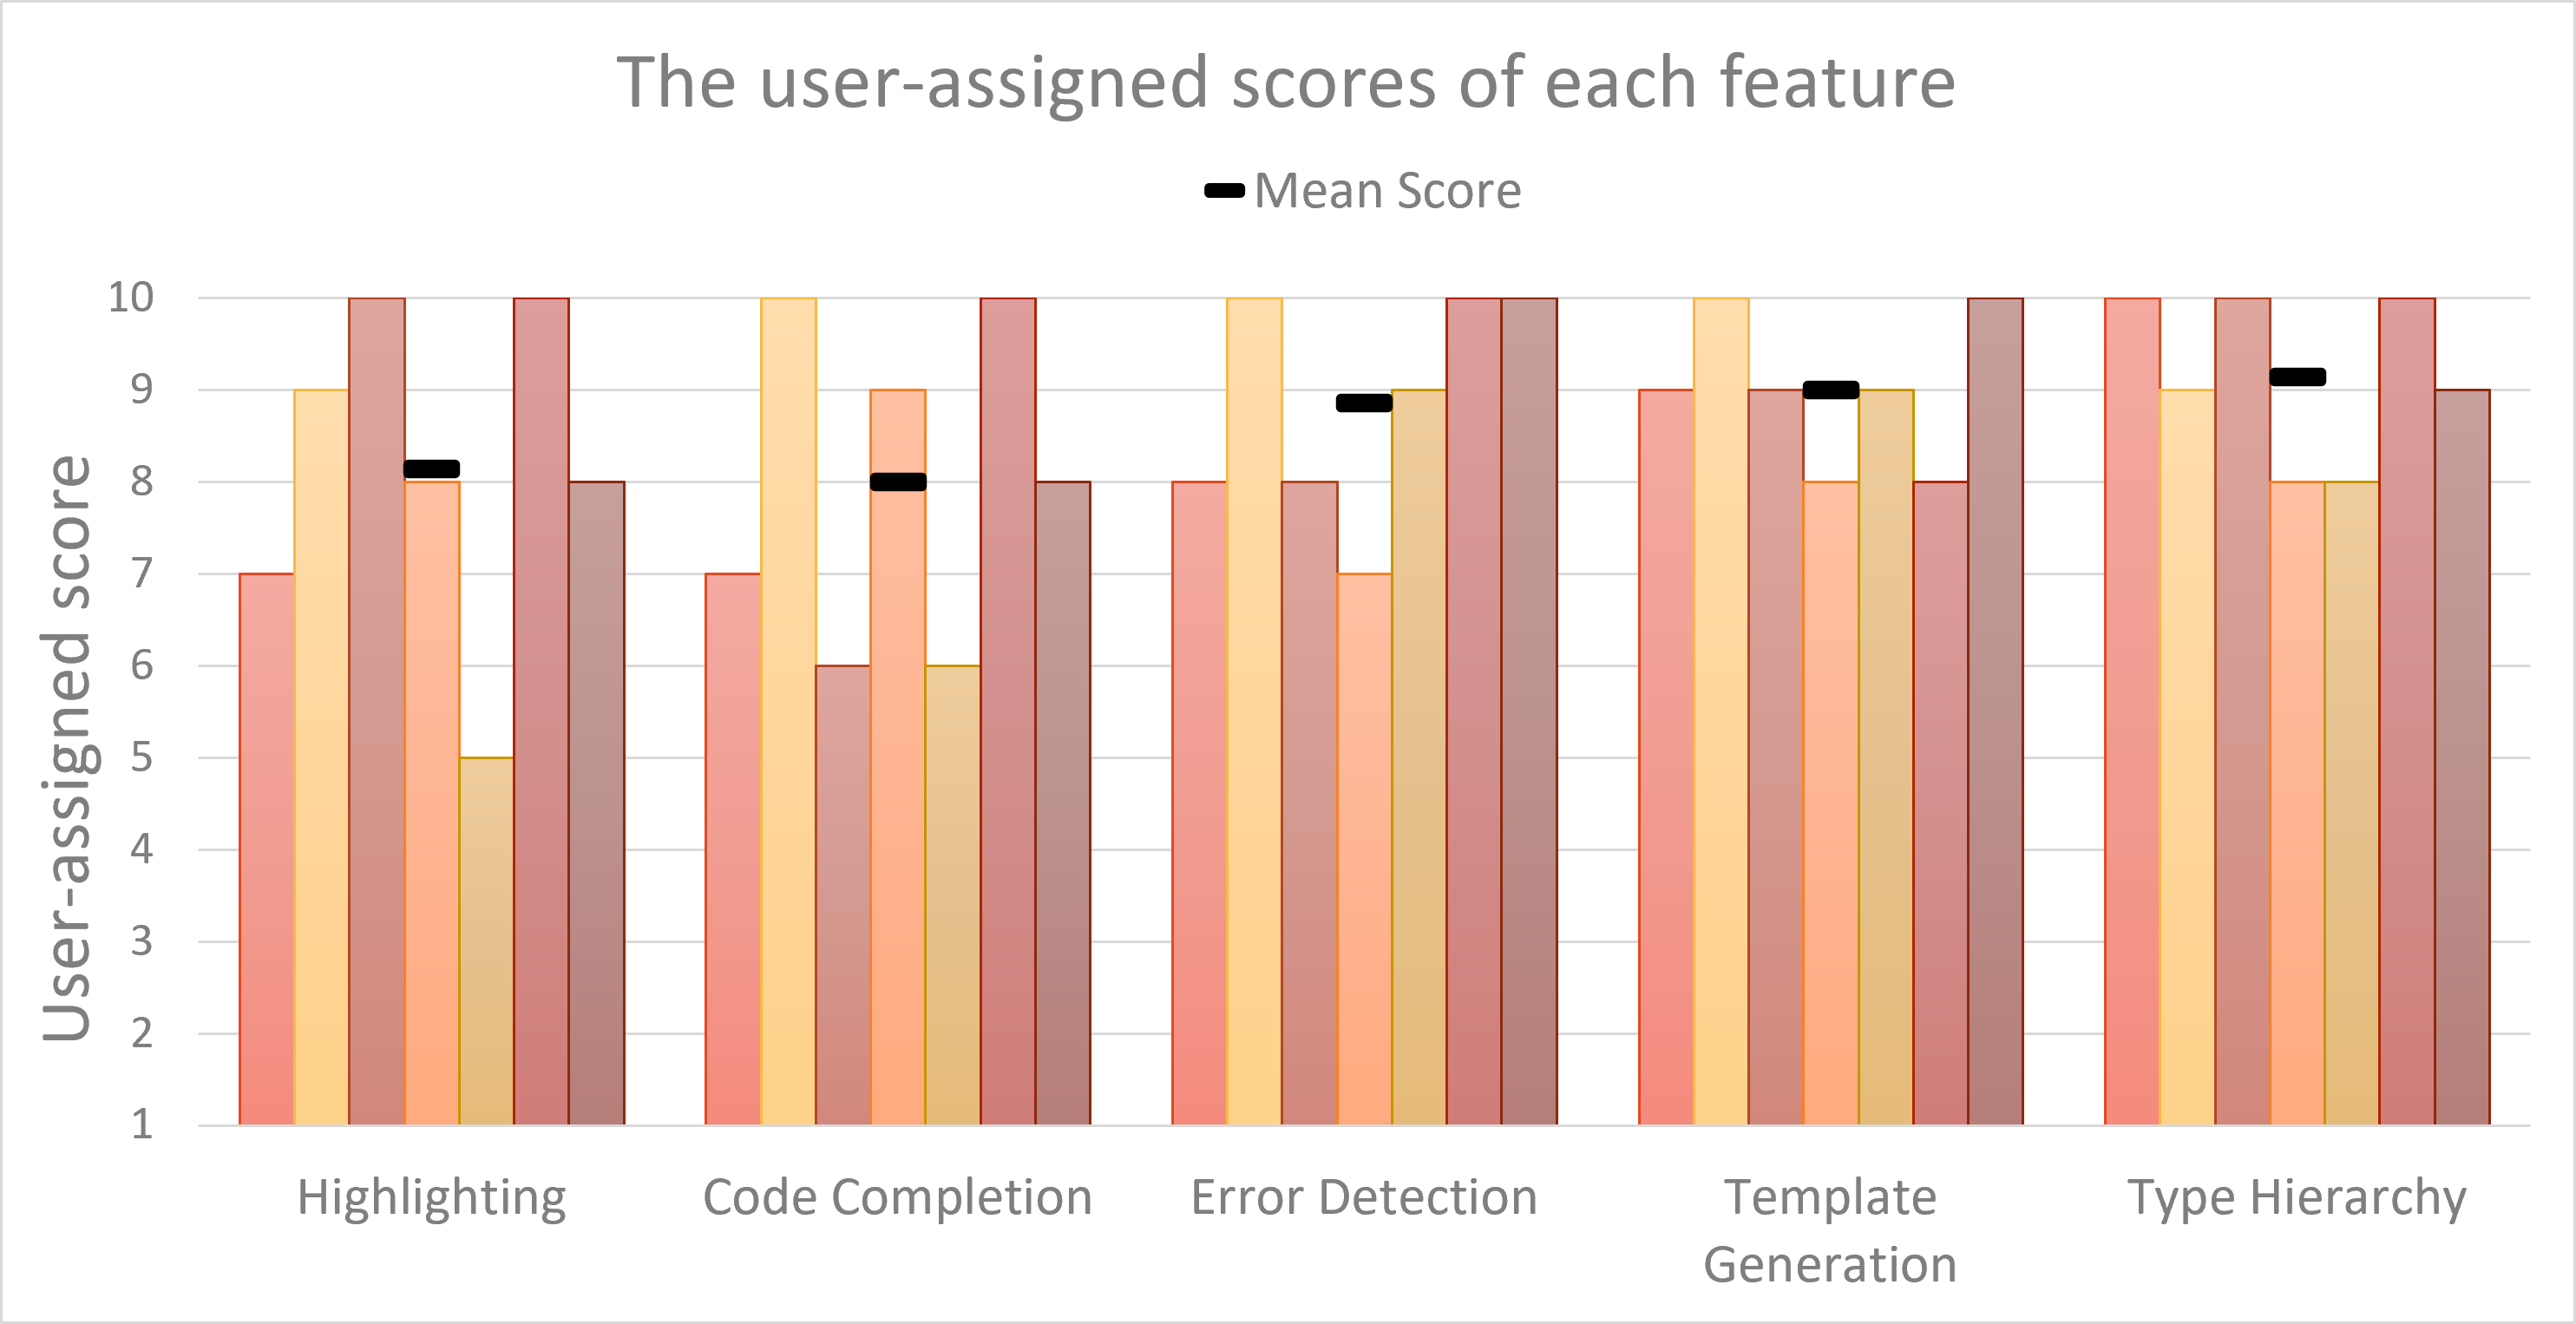
\includegraphics[width = \linewidth]{figures/features-hist-2.png}
\caption{The scores assigned to each feature from a survey with 7 participants. The features are scored by their intuitiveness and usefulness from 1 to 10, with a higher score meaning that a feature is more intuitive and useful.}
\label{fig:scores}
\end{figure}
Figure \ref{fig:scores} shows that each feature was overall rated as highly intuitive and useful, with each feature receiving an average score of no less than 8 out of 10. However, there is a large difference in the scores given to the highlighting and code completion features, with the scores for highlighting ranging from 5 to 10, and the scores for code completion ranging from 6 to 10. This is surprising; I expected the template generation and type hierarchy features, which were more experimental, to receive the lower scores, if any. This result is due to some users encountering minor errors with the features, as explained in their comments about the editor.
% \todo[inline]{Talk about how these issues arent central to the editor, so were only found by some.}
% \todo[inline]{Talk about the positive comments also.}

\subsection{Feedback Comments}
Although the editor was tested heavily before being submitted for review, the form responders encountered some minor issues when testing the editor. Three issues stood out in particular: problems with highlighting unsaved documents, auto-completing section headers and irrelevant code completions being suggested.

\subsubsection{Overall comments}
The comments that the editor received were overall positive. Users were surprised at the intuitiveness of the template auto-generation, especially at the the use of template refinement to give the template accurate variable names. Some users, especially those with little programming experience, found the need for a type hierarchy difficult to understand at first. This was despite the form's example of the type hierarchy being necessary to fix a type mismatch error that should not occur. However, once the type hierarchy was understood, those users found it quite intuitive to write, especially when they experimented with their own examples afterwards. The overall popularity of these two features is evidenced also by their scores, with the two features both scoring an average of approximately 9 out of 10, and no score being lower than 8 out of 10.
\\
\\
The scores given to highlighting and code completion contrast with the scores of the template generation and type hierarchy. This is because some users reported two issues with the features: unsaved documents receiving no highlighting, and erroneous auto-completion for section headers.

\subsubsection{Highlighting unsaved documents}
Visual Studio Code allows the user to write in a new document before it is saved. The logical english editor is usually activated when a file is given the \codeword{.le} file extension. However, it can also be manually activated by the user on unsaved documents. The language client is not started in this scenario. This means that the only features the document receives is highlighting from the syntax highlighter \footnote{Juding by how the other features scored highly, I assume that the users who encountered this issue then tried saving the document, which caused the language server to start and the rest of the features to activate.}.
\\
\\
On investigating the issue, I found that the issue is reproducible on both Windows and Ubuntu Linux platforms. The language client documentation does not mention this issue and, as found through preliminary testing, the TypeScript language extension does not suffer from this issue either. Investigating this issue further is left for future work.

\subsubsection{Auto-Completing Section Headers}
To make writing the document easier for new users, I added the ability to auto-complete the section headers \codeword{the type hierarchy is:}, \codeword{the templates are:}, and \codeword{the knowledge base __ includes:}, where on selecting the latter suggestion, the user is taken to the \codeword{_} to fill the name of the knowledge base in. However, selecting the suggestion \codeword{the type hierarchy is:} lead to the section header \codeword{the templates are:} being written. This was a simple mistake on my part which was quickly fixed.


\section{Automated Testing}
Once the editor had been adjusted in light of the user feedback, the functionality and correctness of the editor were assessed with automated tests. With automated testing, the thoroughness and certainty of the tests can be verified by other testers. The tests can also be carried out to test backwards compatibility if the editor is developed further.

\subsection{Functionality Tests}
End-to-end tests are used to test the editor's functionality. The highlighting, diagnostics, code completion and quick-fix functionalities are tested through a total of 21 end-to-end test cases. 
\\
\\
These tests tested the editor's functionality from the user's perspective. In each test case, the editor opens a Logical English program. The editor's behaviour when providing a feature is then queried and checked against the desired behaviour.
\\
\\
The editor is tested in every feature listed in Section \ref{section:project-requirements} against its required behaviour. These features are tested in areas of standard use: each test case examines the editor's behaviour when editing a realistic Logical English document. These test cases cannot claim to be exhaustive, since Logical English's grammar is not specified to a level of detail that determines edge cases. However, the end-to-end tests test both  ``complex'' features of Logical English, such as type hierarchies and higher-order atomic formulas.

\subsection{Correctness Tests}
Unit tests are used to test the correctness of the language server. The behaviour of the two most complex classes, \codeword{Template} and \codeword{TypeTree}, is tested with 25 unit tests. These tests are supplemental to the end-to-end tests. Since the behaviour of Logical English has not been specified in edge cases, the unit tests are used to determine whether the \codeword{Template} and \codeword{TypeTree} classes can handle edge cases in their input. This allows the editor to be easily updated to incorporate a more specific grammar.

\subsection{Test Results}
The editor passes each of the 21 end-to-end tests. The language server passes each of the 25 unit tests.
\end{document}